% THIS IS AN EXAMPLE DOCUMENT FOR VLDB 2012
% based on ACM SIGPROC-SP.TEX VERSION 2.7
% Modified by  Gerald Weber <gerald@cs.auckland.ac.nz>
% Removed the requirement to include *bbl file in here. (AhmetSacan, Sep2012)
% Fixed the equation on page 3 to prevent line overflow. (AhmetSacan, Sep2012)

\documentclass{sig-alternate}
\usepackage{graphicx}
\usepackage{color}
\usepackage{balance}  % for  \balance command ON LAST PAGE  (only there!)
\usepackage{times}
\usepackage{url}
\usepackage{algorithm}
\usepackage[noend]{algorithmic}
\usepackage{subfigure}
\usepackage{xspace}
\usepackage[noend]{algorithmic}
\usepackage{enumerate}
\usepackage{multirow}
\usepackage{epstopdf}
\usepackage{cleveref}
\newcommand{\squishlist}{
   \begin{list}{$\bullet$}
    {
      \setlength{\itemsep}{0pt}
      \setlength{\parsep}{3pt}
      \setlength{\topsep}{3pt}
      \setlength{\partopsep}{0pt}
      \setlength{\leftmargin}{1.5em}
      \setlength{\labelwidth}{1em}
      \setlength{\labelsep}{0.5em} } }

\newcommand{\squishend}{
    \end{list}  }

\newcommand{\argmax}{\operatornamewithlimits{arg\ max}}

\newcommand{\eat}[1]{}
\newcommand{\todo}[1]{\textcolor{red}{{TODO: #1}}}
\newcommand{\add}[1]{\textcolor{red}{{ADD: #1}}}
\newcommand{\note}[1]{\textcolor{blue}{{#1}}}

\newtheorem{definition}{Definition}
\newtheorem{example}{Example}
\newtheorem{theorem}{Theorem}
\newtheorem{lemma}{Lemma}
\newtheorem{problem}{Problem}
\newtheorem{reduction}{Reduction}
\newcommand{\domain}{\mathcal{D}}
\newcommand{\attributes}{\mathcal{A}_D}
\newcommand{\hierarchy}{\mathcal{H}_D}
\newcommand{\attrhierarchy}{\mathcal{H}_A}
\newcommand{\workers}{\mathcal{W}}
\newcommand{\uentities}{\mathcal{E}}
\newcommand{\queryvector}{{\bf Q_S}}



\begin{document}

% ****************** TITLE ****************************************

\title{CrowdGather: Budgeted Entity Extraction over Structured Data Domains}

\numberofauthors{3} 

\author{
}

\maketitle

\begin{abstract}
Crowd entity extraction has become a popular means of acquiring data for many applications, including recommendation systems, listing aggregation and knowledge base compilation.  Most of the current solutions focus on entity extraction for specific queries and do not consider entity extraction over broader entity domains. Due to the time and cost of human labor, considering each query in isolation may incur large costs when applied to broader domains, thus, limiting the applicability of current approaches.
 
In this paper, we explore the problem of {\em budgeted entity extraction} over {\em structured entity domains}. We consider domains that can be fully described by a collection of attributes, each characterized by a hierarchical structure. We develop new statistical tools that enable users to reason about the gain of issuing {\em further queries} in the presence of little information and show how to exploit the dependencies across different points of the data domain to obtain more accurate estimates. We also demonstrate how budgeted entity extraction over large domains can be cast as an adaptive optimization problem that seeks to maximize the number of extracted entities while minimizing the overall extraction cost. We evaluate our techniques with experiments on both synthetic and real-world data. 
\end{abstract}

\section{Introduction}
\label{sec:intro}
Combining human computation with traditional computer systems has been recently proven beneficial in extracting knowledge and acquiring data for many application domains, including recommendation systems~\cite{amsterdamer:2014}, knowledge base completion~\cite{kondredi:2014}, entity extraction and structured data collection~\cite{trushkowsky:2013, park:2014}. In fact, extracting information, and entities in particular, from the crowd has been shown to provide access to more fine grained information that may belong to the long tail of the web or even be completely unavailable on the web~\cite{west:2014}.

A fundamental challenge in crowd entity extraction is reasoning about the completeness of the extracted information. More precisely, given a query that seeks to enumerate entities from a specific domain, how can one decide on the completeness of the retrieved entities. Recent work has considered this problem for single queries~\cite{trushkowsky:2013} where the query predicates specify the data domain of interest. Often, however, crowd entity extraction techniques are used to acquire information for large data domains that cannot be described adequately by a single query with fixed predicates. Consider for example a scenario where crowd sourcing techniques are used to collect information about various types of events (e.g., music concerts or political rallies) over different countries. Extracting entities from this domain requires issuing multiple targeted queries requesting the crowd to provide information for specific types of events potentially focusing on a specific location. Crowd entity extraction in such domains entails several challenges. Next, we use a real-world scenario to illustrate these challenges.

\subsection{Challenges and Opportunities}
\label{sec:challenges}
We consider Eventbrite~\footnote{https://www.eventbrite.com}, an online event aggregator, that relies on crowdsourcing to compile a directory of events with detailed information about the location, type, date and category of each event. Typically, event aggregators are interested in collecting information about diverse events spanning from conferences and music festivals to political rallies for multiple locations across different location, i.e., countries or cities. In particular, Eventbrite collects information about events across different countries in the world. Each country is further split into cities and areas across the country. Moreover, events are organized according to their type and topic. Eventbrite uses 20 different types to characterize events, such as rallies, tournaments, conferences, conventions, etc. and 20 different topics, such as government and politics, health and wellness, music, etc.  to describe each event. Each topic is further split into sub-topics. For example, a  music event can be further described according to its corresponding genre. 

\textcolor{red}{I want to fill this out with plots of eventbrite events. I will use the eventbrite API and create the plots}

\ \\First challenge: sparse areas of the data domain. Given a budget might not worth be issuing any queries to extract more events there
\ \\Add a plot showing that for certain location, event type, topic combinations there are no events or a much smaller number of events. 

\ \\Opportunity: Exploit the hierarchical structure of the data domain. Discuss how the structure of Eventbrite's hierarchy can be exploited to discover sparse areas and optimize for the budget.

\ \\Second challenge: Side information. Show example of overlaps. and the fact that when we request events for a location we get many events for a specific topic etc. dependent samples.

\subsection{Contributions}
\label{sec:contributions}
Motivated by these examples, we study the problem of {\em budgeted crowd entity extraction} over {\em structured domains}. More precisely, we focus on domains described by a collection of attributes, each following a known hierarchical structure. We assume that for each attribute the corresponding hierarchy is known. Moreover, we assume that after issuing a query against the crowd the retrieved answers can be associated with all relevant nodes across all attribute hierarchies, i.e., a worker will provide all the attribute values describing a reported entity. Dealing with incomplete information about entities is not the main focus of this paper and is part of the future work preposed in \Cref{sec:conclusions}/

We propose a novel algorithmic framework that exploits the structure of the domain to maximize the number of extracted entities under given budget constraints. In particular, we view the problem of entity extraction as a {\em multi-round adaptive optimization problem}. At  each round we exploit the information on extracted entities obtained by previous queries to adaptively select the crowd query that will maximize the {\em gain} and cost trade-off at each round. The gain of a query is defined as the number of new unique entities extracted by it. Building upon techniques from the species estimation literature, we introduce a new methodology for estimating the gain for generalized queries and show how the hierarchical structure of the domain can be exploited to improve the accuracy of our estimates. Our main contributions are as follows:

\squishlist
\item We study the problem of budgeted entity extraction over structured domains and show how one can exploit the domain structure to maximize the set of extracted entities under budget constraints. 
\item We develop a new technique to estimate the gain of generalized entity extraction queries under the presence of dependent samples.
\item We introduce an adaptive optimization algorithm that takes as input the gain estimates for different types of queries and identifies querying policies that maximize the total number of retrieved entities under given budget constraints. 
\item Finally, we show that our techniques can effectively solve the problem of budgeted crowd entity extraction for large data domains on both real-world and synthetic data.
\squishend

\section{Preliminaries}
\label{sec:prelims}
In this section we first review the problem of {\em crowdsourced entity extraction over structured domains} under budget constraints. Then, we review different types of crowd queries for entity extraction.

\subsection{Crowd Entity Extraction}
\label{sec:extraction}
Let $\domain$ be a data domain described by a set of discrete attributes $\attributes = \{A_1, A_2, \dots, A_d\}$. Let $dom(A_i)$ denote the domain of each attribute $A_i  \in \attributes$. We focus on structured domains where each attribute is hierarchically organized. For example, consider the event domain introduced in \Cref{sec:challenges}. The data domain $\domain$ corresponds to all events and the attributes describing the entities in $\domain$ are $\attributes = \{$``Event Type", ``Event Topic", ``Location", ``Date"$\}$. \Cref{fig:eventsdomain} shows the hierarchical organization of each attribute.

\begin{figure}
	\begin{center}
	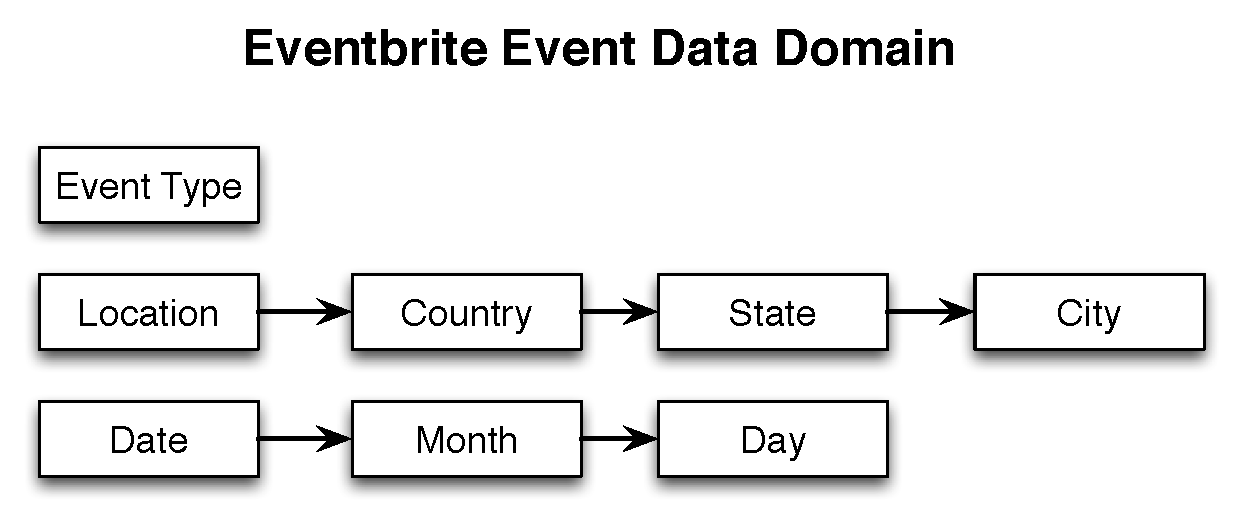
\includegraphics[clip,scale=0.4]{figs/eventsDomain.eps}
	\caption{The attributes describing the events domain and the hierarchical structure of each attribute.}
	\label{fig:eventsdomain}
	\end{center}
\end{figure}

The domain $\domain$ can be viewed as a {\em lattice} corresponding to the crossproduct of all available hierarchies. Part of the lattice corresponding to the previous example is shown in \Cref{fig:eventslattice}. We denote this crossproduct as $\hierarchy$. We define a {\em point} in $\domain$ as a possible combination of values of {\em all} attributes. We will also refer to a collection of points for which only a subset of attributes shares the same value as a {\em slice} $\domain_P$ of $\domain$. For example, a slice of the event domain described above may correspond to rock concerts in Boston. The predicates describing this slice are EVENT TYPE = ``Concert", EVENT TOPIC=``Music, Rock", LOCATION = ``Boston, MA", DATE = ``*".  It is easy to see that each node in $\hierarchy$ represents a slice of the data domain $\domain$. 

\begin{figure}
	\begin{center}
	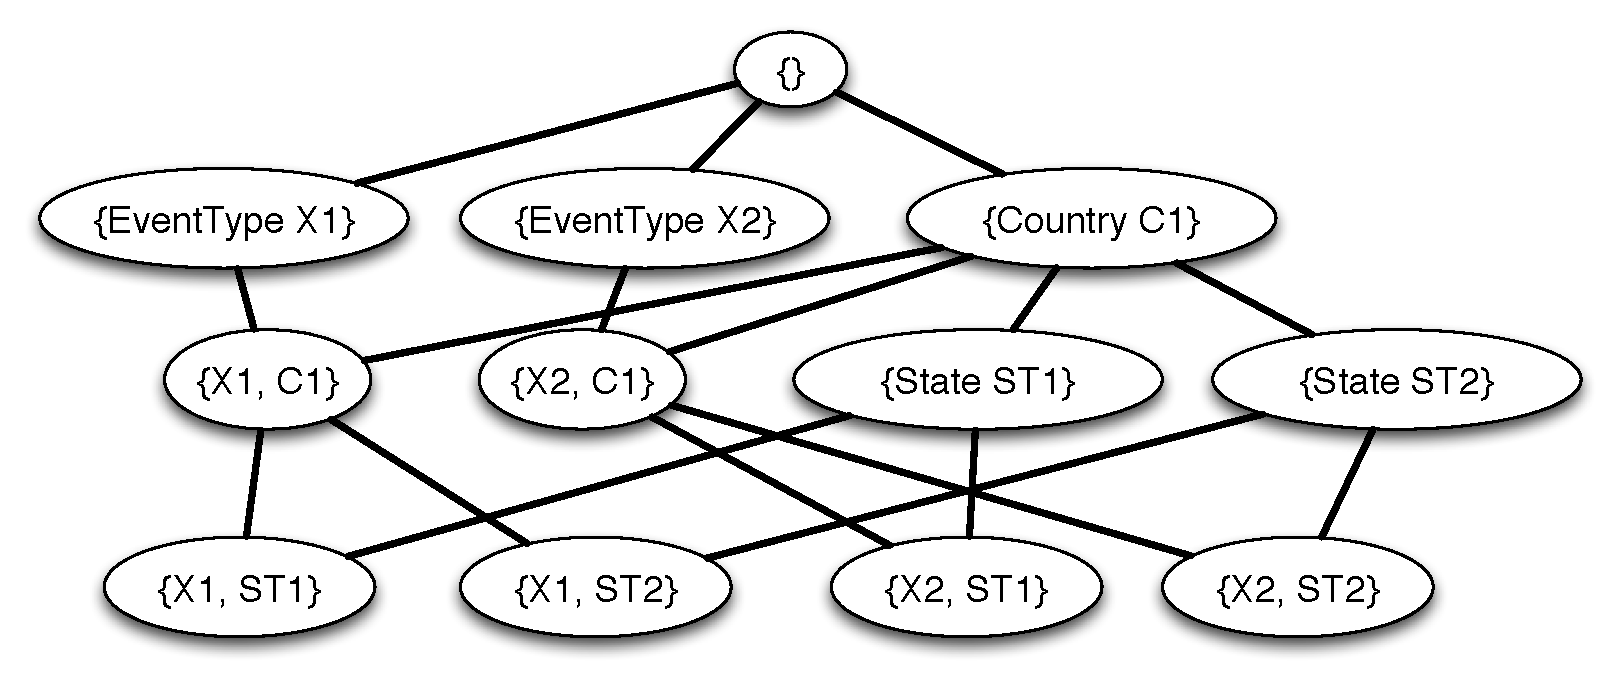
\includegraphics[clip,scale=0.35]{figs/eventsExLattice.eps}
	\caption{Part of the lattice defining the entire event entity domain described by the attributes in \Cref{fig:eventsdomain}.}
	\label{fig:eventslattice}
	\end{center}
\end{figure}

The basic version of {\em crowd entity extraction}~\cite{trushkowsky:2013} seeks to extract entities that belong in a {\em single} slice $\domain_P$ of $\domain$, specified by a set of predicates $P$ over a subset of attributes in $\attributes$. However, when considering large entity domains, such as the event domain, one may need to issue a series of entity extraction queries over multiple slices of $\domain$ - that may overlap with each other- so that the entire domain is covered. Issuing queries for different slices of the domain ensures that the coverage across the domain will be maximized. 

Let $\mathcal{P}(\domain)$ denote the set of all possible slices that their union covers the domain $\domain$. Moreover, let $\pi$ denote a {\em querying policy}, that is, a chain of crowd queries corresponding to different slices in $\mathcal{P}(\domain)$. Each query asks workers to provide entities corresponding to a slice $\domain_P$. Notice, that multiple queries can be issued against the same slice. Let $C(\pi)$ denote the overall cost, both in terms of monetary cost and latency, of a querying policy $\pi$. We define the gain of a querying policy $\pi$ as the total number of unique entities, denoted by $\uentities(\pi)$ extracted when following policy $\pi$. 

The above naturally gives raise to a tradeoff between the total number of extracted entities and the total cost. To optimize this tradeoff, previous work has proposed either a {\em pay-as-you-go} scheme~\cite{trushkowsky:2013} or a fixed answer size scheme~\cite{park:2014}. In the first case, one repeatedly issues queries to the crowd until the {\em marginal gain}, i.e., the difference between the new extracted entities and the querying cost, drops below a desired threshold. However, the proposed scheme does not enforce any budget constraints explicitly and focuses on a single query in isolation. Thus, it does not optimize the gain-cost tradeoff over an entire querying policy. In the second case, one repeatedly issues queries to the crowd until a desired number of entities is retrieved. The latter is specified by the user. Notice, that this assumes knowledge of the number of entities to be extracted, nevertheless, this information may not be available in many real-world scenarios. 

Here, we require that the user will {\em only} provide a monetary budget $\tau_c$ imposing a constraint on the total cost of a selected querying policy, and optimize over all possible querying policies across different slices of the data domain. Our goal is to identify the policy that maximizes the number of retrieved entities under the given budget constraint. More formally, we define the problem of budgeted crowd entity extraction as follows:

\begin{definition}[Budgeted Crowd Entity Extraction]
Let $\domain$ be a given entity domain and $\tau_c$ a monetary budget on the total cost of issued queries. The Budgeted Crowd Entity Extraction problem seeks to find 
a querying policy $\pi^*_S$ over a subset of slices $S \subseteq \mathcal{P}(\domain)$ that maximizes the number of unique entities extracted $\uentities(\pi^*_S)$ under the constraint $C(\pi^*_S) \leq \tau_c$.
\end{definition}

If $\domain$ is fully specified by a hierarchy $\hierarchy$ then $\mathcal{P}(\domain) = \hierarchy$. Thus, determining the optimal querying policy requires detecting the optimal subset of nodes in $\hierarchy$ to be queried so that the goal number of extracted entities is maximized under the given budget constraint. In the reminder of the paper we focus on queries over nodes of $\hierarchy$.

The cost of a querying policy $\pi$ is defined as the total cost of all queries issued by following $\pi$. We have that $C(\pi) = \sum_{q \in \pi} c(q)$ where the cost of each query $q$ is defined according to a cost model specified by the user. Computing the total cost of a policy $\pi$ is easy. However, the gain $\uentities(\pi)$ of a policy $\pi$ is unknown as we do not know in advance the entities corresponding to each node in $\hierarchy$, and hence, needs to be estimated, as we discuss in \Cref{sec:gain}. 

\subsection{Entity Extraction Queries}
\label{sec:queries}
We consider three different types of crowd queries for answering an entity extraction problem as the one described above. The first type corresponds to {\em single entity queries} where workers are required to provide ``one more" entity that satisfies the query predicates. The second type of queries corresponds to {\em queries of  size k} where workers are asked to provide up to $k$ distinct entities. Finally, the last type corresponds to {\em exclude list queries}. Here,  workers are provided with $l$ entities that have already been extracted and are required to provide up to $k$ distinct entities under the constraint that none of them is included in the exclude list. It is easy to see that the last type of queries generalizes the previous two. Therefore, in the remainder of the paper, we will consider that all queries of the third type. To describe a query, we will use the notation $q(k,l)$ denoting a query of size $k$ accompanied with an exclude list of length $l$. Notice that due to the different query configurations the optimal querying policy for the problem of budgeted crowd entity extraction needs to be redefined. In fact, apart from determining the optimal subset of nodes in $\hierarchy$ to be queried, an optimal querying policy needs to identify the optimal query configurations $q(k,l)$ for each query.

Assuming an infinite pool of crowd workers,  one can extract entities satisfying a set of desired predicates by repeatedly asking workers queries with different configurations $q(k,l)$ across {\em multiple rounds}. However, in a typical crowdsourcing environment, tasks have different costs depending on their difficulty. Thus, crowdsourced queries of different difficulties should also exhibit different costs. Given a query $q(k,l)$, we assume that the cost function $c(\dot)$ obeys the following properties: (a) given an exclude list of fixed length $l$ then $c(q(k^{\prime},l)) \geq c(q(k,l)),  \forall k^{\prime} \geq k$, and (b) given a fixed query size $k$ then $c(q(k,l^{\prime})) \geq c(q(k,l)), \forall l^{\prime} \geq l$. 


\section{Framework Overview}
\label{sec:framework}
In this section, we present an overview of our proposed framework for solving the problem of budgeted crowd entity extraction over structured domains. We argue that the optimization problem described in \Cref{sec:extraction} consists of two subproblems: 
\squishlist 
\item \textbf{Estimating the Gain for a Query.} Given the extracted entities associated with different nodes in $\hierarchy$ we need to estimate the number of new unique entities that will be retrieved for different query configurations $q(k,l)$ at different nodes of $\hierarchy$. 
\item \textbf{Detecting the Optimal Querying Policy.} Using the gain estimates from the previous problem as input we need to identify the next query that will maximize the gain with respect to the remaining budget. 
\squishend

Our proposed framework consists of two components, each responsible for solving the aforementioned problem. An interview 

\section{The Gain of Further Queries}
\label{sec:gain}

\section{Finding Optimal Querying Policies}
\label{sec:solving}

\section{Related Work}
\label{sec:related}

\ \\Beth's work
\ \\Tova's work
\ \\CrowdFill work

\section{Conclusions}
\label{sec:conclusions}


\bibliographystyle{abbrv}
\bibliography{crowd_hierarchies}

\end{document}
